%
% einleitung.tex -- Beispiel-File für die Einleitung
%
% (c) 2020 Prof Dr Andreas Müller, Hochschule Rapperswil
%
% !TEX root = ../../buch.tex
% !TEX encoding = UTF-8
%
\section{Numerische Methoden}

Bisher wurden Feldgleichungen und deren Lösungen aus einer theoretischen und abstrakten Perspektive betrachtet.
Dies ist grundlegend für das Verständnis der zugrundeliegenden Konzepte.

Um den praktischen Nutzen dieser mächtigen Theorie jedoch voll auszuschöpfen, ist ein Übergang von dieser idealisierten, kontinuierlichen und grenzenlosen Sichtweise hin zu einer realitätsnahen, diskreten und physikalisch eingeschränkten Betrachtung erforderlich.
Konkret bedeutet dies, dass wir die Feldgleichungen diskretisieren müssen.

Ein prominentes Beispiel dafür ist das numerische Wettermodell des ECMWF (European Centre for Medium-Range Weather Forecasts), das auf Grundlage eines breiten Spektrums aktueller und vergangener Wetterdaten versucht, möglichst präzise Vorhersagen für die kommenden zehn Tage zu treffen.

Als wichtigste und somit einflussreichste Parameter dieses Modells gelten der Luftdruck, die Lufttemperatur, die Windgeschwindigkeit bzw. -richtung, die Luftfeuchtigkeit sowie diverse Niederschlagsparameter \cite{ecmwf2023}.
Diese Messwerte liegen jedoch nur mit begrenzter zeitlicher und räumlicher Auflösung vor.

Sie bestimmen somit die Feinheit des zugrundeliegenden Datenrasters – ein Umstand, der sich später als entscheidend erweisen wird.

\subsection{Diskretisierung statt Interpolation}

Angesichts der Tatsache, dass die Messwerte nur in diskreter Form vorliegen, stellt sich die Frage, warum man nicht versucht, diese durch geeignete Interpolation wieder in ein kontinuierliches Datenset zu überführen, um dann die bekannten kontinuierlichen Gleichungen analytisch auszuwerten.
Diese Fragestellung allein könnte den Umfang dieses gesamten Papers einnehmen.
Daher sollen im Folgenden nur einige ausgewählte, nicht abschließende Aspekte diskutiert werden.

Ein erster wesentlicher Punkt ist, dass Interpolation ein rein mathematisches Verfahren darstellt, das keinerlei physikalische Gesetzmäßigkeiten berücksichtigt.
In der Praxis führt dies dazu, dass verrauschte und durch das Abtasten bereits verfälschte Messwerte durch Interpolation weiter verfälscht werden können.

Eine mögliche Lösung wäre, die Interpolation um ein physikalisches Modell zu erweitern, welches die Lücken auf plausible Weise schließt.
Dabei würde jedoch ein weiteres physikalisches Modell entstehen, das letztlich nur dazu dient, Daten für das eigentliche Modell zu liefern – was den methodischen Aufwand verdoppelt, ohne zwingend zusätzliche Erkenntnisse zu bringen.

Ein weiterer zentraler Vorteil numerischer Verfahren liegt in ihrer Fähigkeit, auch Gleichungen zu lösen, die keine geschlossene analytische Lösung besitzen.
Dies ist insbesondere in der Strömungsmechanik von Bedeutung.
Ein Beispiel dafür ist die Navier-Stokes-Gleichung, welche die Bewegung von Flüssigkeiten und Gasen beschreibt.
Für den allgemeinen dreidimensionalen Fall ist bis heute keine Lösung in geschlossener Form bekannt.

Numerische Verfahren ermöglichen jedoch näherungsweise Lösungen mit vernachlässigbar kleinen Fehlern, sofern geeignete Diskretisierung und Randbedingungen gegeben sind.
Allen klassischen numerischen Methoden zur Lösung partieller Differentialgleichungen ist gemeinsam, dass sie das kontinuierliche, analytische Problem in ein algebraisches Gleichungssystem mit endlich vielen Unbekannten überführen.
Dieses lässt sich anschließend mit numerischen Verfahren der linearen Algebra effizient auf dem Computer lösen.

\subsection{Überblick über numerische Methoden zur Lösung von Feldgleichungen}

Zur numerischen Lösung partieller Differentialgleichungen existieren verschiedene etablierte Methoden, die je nach Anwendungsgebiet unterschiedliche Vor- und Nachteile aufweisen.
Drei der wichtigsten Verfahren werden im Folgenden kurz vorgestellt.

\subsubsection{Finite-Differenzen-Methode (FDM)}
\label{parallelisierung:section:fdm}

Die Finite-Differenzen-Methode ersetzt Ableitungen durch Differenzenquotienten auf einem diskreten Gitter.
Dadurch wird die ursprüngliche Differentialgleichung in ein algebraisches Gleichungssystem überführt, das die gesuchte Lösung an diskreten Gitterpunkten beschreibt.
FDM ist insbesondere für einfache Geometrien und regelmäßige Gitter gut geeignet und vergleichsweise leicht zu implementieren.
Sie wird häufig bei Wärmeleitungsproblemen, Diffusionsprozessen und einfachen Wellengleichungen verwendet.

\subsubsection{Finite-Elemente-Methode (FEM)}

Die Finite-Elemente-Methode basiert auf der schwachen Formulierung der Gleichung und verwendet eine Zerlegung des Lösungsgebiets in sogenannte Elemente (z.B. Dreiecke oder Tetraeder).
Innerhalb dieser Elemente wird die Lösung durch geeignete Basisfunktionen approximiert.
FEM ist besonders leistungsfähig für komplexe Geometrien, Materialinhomogenitäten und Randwertprobleme in der Elektrotechnik und Strömungsmechanik.

\subsubsection{Finite-Volumen-Methode (FVM)}

Die Finite-Volumen-Methode basiert auf der integralen Form der Erhaltungssätze (z.B. Massen-, Impuls- oder Energieerhaltung) und ist besonders geeignet für konservative Systeme, also Systeme, bei denen physikalische Erhaltungsgrößen wie Masse oder Energie nicht erzeugt oder vernichtet, sondern nur transportiert oder umgewandelt werden.
Die Methode berechnet Flüsse über die Ränder sogenannter Kontrollvolumina.
Sie ist weit verbreitet in der Computational Fluid Dynamics (CFD), insbesondere bei der Simulation von Strömungen, Gasdynamik und Transportprozessen.

\subsubsection{Wahl der Methode}

Für das im Folgenden betrachtete Beispiel – die eindimensionale Wärmeleitungsgleichung – ist die Finite-Differenzen-Methode besonders geeignet.
Die Geometrie ist einfach, und das Verfahren erlaubt eine direkte, transparente Umsetzung der zugrundeliegenden physikalischen Zusammenhänge in eine diskrete Form.
Daher wird im nächsten Abschnitt die FDM im Detail erläutert und anhand eines konkreten Beispiels demonstriert.

\subsection{Beispiel FDM}

Als Ausgangslage wird die allgemeine Wärmeleitungsgleichung
\begin{equation}
	\frac{\partial T}{\partial t}
	=
	\alpha \Delta T.
	\label{parallelisierung:eq:Wärmeleitung_alg}
\end{equation}
betrachtet.
Im folgenden wird im 2D-Raum gearbeitet, also resultiert
\begin{equation}
	\frac{\partial T}{\partial t}
	=
	\alpha \left(
	\frac{\partial^2 T}{\partial x^2}
	+
	\frac{\partial^2 T}{\partial y^2}
	\right).
	\label{parallelisierung:eq:Wärmeleitung_2D}
\end{equation}


\subsubsection{Diskretisierung der Variablen}

Als erstes müssen die Variablen diskretisiert werden. Dies tun wir indem wir ein Gitter über den gesamten Bereich (zeitlich, sowie räumlich) legen, also
Im Raum:
\begin{equation}
	x_i
	=
	i \cdot \Delta x,
\end{equation}
\begin{equation}
	y_j
	=
	j \cdot \Delta y,
\end{equation}
und in der Zeit:
\begin{equation}
	t_n
	=
	n \cdot \Delta t.
\end{equation}

Somit wird unsere resultierende, diskrete Temperaturfunktion die Form
\begin{equation}
	T^n_{i,j}
	=
	T(x_i,y_j,t_n)
\end{equation}
haben.


\subsubsection{Diskretisierung der Zeit}

Die partielle Ableitung der Temperaturfunktion \( T \) nach der Zeit wird durch eine explizite Vorwärtsdifferenz approximiert:

\begin{equation}
	\label{parallelisierung:eq:discrete_time_derivative}
	\left. \frac{\partial T}{\partial t}\right|{(i,j,n)}
	\approx
	\frac{T_{i,j}^{n+1} - T_{i,j}^n}{\Delta t}.
\end{equation}
Dies entspricht der zeitlichen Änderungsrate von \( T \) am diskreten Gitterpunkt \( (x_i, y_j, t_n) \).

\subsubsection{Diskretisierung des Raums}
Auch hier beginen wir mit der einmaligen Anwendungen des Differentialquotienten (vorwärts), um die erste Ableitung, zunächst in $x$-Richtung zu approximieren:

\begin{equation}
	\left. \frac{\partial T}{\partial x} \right|{(i,j,n)}
	\approx \frac{T_{i+1,j}^n - T_{i,j}^n}{\Delta x}.
\end{equation}
Zusätzlich bestimmen wir den Differentialquotienten an einem vorangehenden Gitterpunkt
\begin{equation}
	\left. \frac{\partial T}{\partial x} \right|{(i-1,j,n)}
	\approx \frac{T_{i,j}^n - T_{i-1,j}^n}{\Delta x},
\end{equation}
um mittels einer letzen Anwendung des Differentialquotienten die Änderung dieser beiden Änderungen, also genau das was die zweite Ableitung beschreibt, diskret zu bestimmen
\begin{equation}
	\frac{\partial^2 T}{\partial x^2} \approx
	\frac{ \left( \frac{T_{i+1,j}^n - T_{i,j}^n}{\Delta x} \right) - \left( \frac{T_{i,j}^n - T_{i-1,j}^n}{\Delta x} \right) }{\Delta x}.
\end{equation}
Schlussendlich vereinfacht sich dies zu 
\begin{equation}
	\label{parallelisierung:eq:discrete_x_derivative}
	\left. \frac{\partial^2 T}{\partial x^2} \right|{(i,j,n)} \approx \frac{T_{i+1,j}^n - 2T_{i,j}^n + T_{i-1,j}^n}{(\Delta x)^2}.
\end{equation}
Für die y-Richtung folgt analog
\begin{equation}
	\label{parallelisierung:eq:discrete_y_derivative}
	\left. \frac{\partial^2 T}{\partial y^2} \right|{(i,j,n)} \approx \frac{T_{i,j+1}^n - 2T_{i,j}^n + T_{i,j-1}^n}{(\Delta y)^2}.
\end{equation}


Nun setzen wir die in den Formeln \eqref{parallelisierung:eq:discrete_time_derivative},  \eqref{parallelisierung:eq:discrete_x_derivative} und \eqref{parallelisierung:eq:discrete_y_derivative} gefundenen Gleichungen in die Ursprüngliche zweidimensionale Wärmeleitungsgleichung Formel \eqref{parallelisierung:eq:Wärmeleitung_2D} ein.
Somit erhalten wir 

\begin{equation}
	\label{parallelisierung:eq:update_formula_unsorted}
	\frac{T_{i,j}^{n+1} - T_{i,j}^n}{\Delta t}
	=
	\alpha \left(
	\frac{T_{i+1,j}^n - 2 T_{i,j}^n + T_{i-1,j}^n}{(\Delta x)^2}
	+
	\frac{T_{i,j+1}^n - 2 T_{i,j}^n + T_{i,j-1}^n}{(\Delta y)^2}
	\right),
\end{equation}
womit die diskretisierung der Wärmeleitungsgleichung mittels der Finite-Differenzen-Methode gezeigt ist.

\subsubsection{Explizite Updateformel}
\label{parallelisierung:sec:update_formel}


Aufgrund der lokalität und kausalität der Feldgleichungen ist die Temperatur eines Gitterpunkts \( (x_i, y_j)\) zu einem bestimmten Zeitpunkt in der Zukunft \( (t_n)\) sprich \(T_{i,j}^{n+1}\) nur von dem  vorangegangenen Zustand eben dieses Gitterpunkts und desen direkten Nachbbaren abhängig.
Dies ist  in der nach \(T_{i,j}^{n+1}\) umgestellten Formel (\ref{parallelisierung:eq:update_formula_unsorted}) ersichtlich:
\begin{equation}
	\label{parallelisierung:eq:update_formula_sorted}
	T_{i,j}^{n+1}
	=
	T_{i,j}^n
	+
	\alpha \, \Delta t \left(
	\frac{T_{i+1,j}^n - 2 T_{i,j}^n + T_{i-1,j}^n}{(\Delta x)^2}
	+
	\frac{T_{i,j+1}^n - 2 T_{i,j}^n + T_{i,j-1}^n}{(\Delta y)^2}
	\right)
\end{equation}

Aus Übersichtsgründen fassen wir alle Konstanten (\(\alpha, \Delta t, \Delta x, \Delta y) \) zu einer neuen Konstanten zusammen.
Als praktische vereinfachung dazu legen wir fest, dass wir mit einem quadratischen Raumgitter arbeiten. Somit setzen wir  \(\Delta l = \Delta x = \Delta y\) und
\begin{equation}
	\label{parallelisierung:eq:lambda}
	\lambda 
	:= 
	\frac{\alpha \Delta t}{(\Delta l)^2}.
\end{equation}

Nun sind wir in der Lage, Formel \eqref{parallelisierung:eq:update_formula_sorted} kompakt und übersichtlich zu schreiben:

\begin{equation}
	\label{parallelisierung:eq:update_formel}
	T_{i,j}^{n+1}
	=
	T_{i,j}^n +
	\lambda \left(
	T_{i+1,j}^n + T_{i-1,j}^n + T_{i,j+1}^n + T_{i,j-1}^n - 4 T_{i,j}^n
	\right).
\end{equation}
Diese Formel wird als explizite Updateformel bezeichent, da sie iterativ auf Grundlage von gemesenen Daten oder zuvor berechneten Datenpunkten den nächsten Zeitschritt auswertet.

Es ist nun klar ersichtlich, dass die Temperatur an einem Punkt (\(x_i, y_j\)) zu einem gegebenen Zeitpunkt \(t_{n+1}\)  von der Temperatur an diesem Punkt zum Zeitpunkt \(t_n\) und der Wärmeflussbilanz zu den 4 direkten Nachbarquadraten abhängig ist.

\subsubsection{Stabilitätskriterien}

Die in Gleichung~\eqref{parallelisierung:eq:lambda} eingeführte dimensionslose Konstante \(\lambda\) entscheidet, 
ob eine explizite FDM-Simulation stabil bleibt.  
Tabelle~\ref{parallelisierung:tab:stabilitaet_fdm} fasst die Stabilitätsbedingungen für Probleme verschiedener 
Dimensionen zusammen, wie sie aus einer Fourier-Analyse des Verstärkungsverhaltens einzelner Fehlerkomponenten 
resultieren.  
Aus Gründen der Lesbarkeit wird die vollständige Herleitung dieser Bedingungen an dieser Stelle nicht wiedergegeben; 
eine historische Einführung findet sich bereits bei Fourier \cite{Fourier1822}, während die systematische 
von-Neumann-Stabilitätsanalyse in \cite{VonNeumann1950} beschrieben ist.

\label{parallelisierung:sec:stabilitaetskriterien}

\begin{table}
	\centering
	\caption{Stabilitätsbedingungen der expliziten Finite-Differenzen-Methode}
	\label{parallelisierung:tab:stabilitaet_fdm}
	\begin{tabular}{|c|c|}
		\hline
		\textbf{Dimension} & \textbf{Stabilitätsbedingung} \\
		\hline
		1 & 
		\( \displaystyle \lambda = \frac{\alpha \, \Delta t}{(\Delta x)^2} \leq \frac{1}{2} \) \\
		\hline
		2 & 
		\( \displaystyle \lambda_x + \lambda_y =
		\frac{\alpha \, \Delta t}{(\Delta x)^2} +
		\frac{\alpha \, \Delta t}{(\Delta y)^2} \leq \frac{1}{2} \) \\
		\hline
		3 & 
		\( \displaystyle \lambda_x + \lambda_y + \lambda_z =
		\frac{\alpha \, \Delta t}{(\Delta x)^2} +
		\frac{\alpha \, \Delta t}{(\Delta y)^2} +
		\frac{\alpha \, \Delta t}{(\Delta z)^2} \leq \frac{1}{2} \) \\
		\hline
	\end{tabular}
\end{table}



Für den zweidimensionalen Fall gilt:
\begin{equation}
	\lambda_x + \lambda_y =
	\frac{\alpha \, \Delta t}{(\Delta x)^2} +
	\frac{\alpha \, \Delta t}{(\Delta y)^2} \leq \frac{1}{2}.
\end{equation}
Mit \(\Delta l = \Delta x = \Delta y\) folgt \(\lambda = \lambda_x = \lambda_y\), sodass sich die Formel zu
\begin{equation}
	2\lambda = 2 \frac{\alpha \, \Delta t}{(\Delta l)^2} \leq \frac{1}{2}
	\quad \Rightarrow \quad
	\lambda = \frac{\alpha \, \Delta t}{(\Delta l)^2} \leq \frac{1}{4}
\end{equation}
ergiebt.

\paragraph{Physikalische Intuition}  
Man kann sich die Wärmeausbreitung wie das Füllen mehrerer miteinander verbundener Wasserbehälter vorstellen.  
Ist der Zeitabstand \(\Delta t\) zwischen den „Kontrollpunkten“ zu groß, können sich die Pegel zwischen den Behältern stark über- oder unterschwingen, anstatt sich gleichmäßig auszugleichen.  
Eine Erhöhung der thermischen Diffusivität \(\alpha\) wirkt ähnlich wie eine Verringerung der Viskosität einer Flüssigkeit: der Ausgleich erfolgt schneller, sodass kleinere Zeitintervalle notwendig werden.  
Auch eine Verringerung von \(\Delta x\) (feinere räumliche Auflösung) erfordert kleinere Zeitschritte, da die Temperaturunterschiede über kürzere Distanzen schneller wirken.
Im folgenden soll anhand von drei Experimenten die stabilität der Simulation, basierend auf der Updateformel  \eqref{parallelisierung:eq:update_formel}, genauer untersucht werden.

\subsubsection{Stabilitätsexperiment}

Zur Demonstration der Stabilitätsbedingung wird folgendes Szenario betrachtet:
Eine \(9 \times 9 \, \mathrm{cm}\) große Stahlplatte (ohne dritte Dimension) befindet sich in einer Umgebung mit konstanter Temperatur von \(0\,^{\circ}\mathrm{C}\).  
Die linke und rechte Kante werden konstant auf \(100\,^{\circ}\mathrm{C}\) gehalten.  
Das Material besitzt die Eigenschaften:
\begin{center}
	\begin{tabular}{llll}
		Wärmeleitfähigkeit & \(\kappa\) & 50 &
		\(\mathrm{W/(m \cdot K)}\) \\
		Dichte & \(\rho\)   &  7850 & \(\mathrm{kg/m^3}\) \\
		spezifische Wärmekapazität & \(c\) &  470 & \(\mathrm{J/(kg \cdot K)}\)
	\end{tabular}
\end{center}
Somit ergibt sich die thermische Diffusität zu


\[
\alpha =
\frac{\kappa}{\rho c}
=
\frac{50}{7850 \cdot 470}
= 1.355 \cdot 10^{-5}.
\]

\paragraph{Fall 1: Stabile Simulation}  
Mit \(100\) Messpunkten in einem \(10\times 10\)-Raster beträgt der Abstand \(\Delta l = 0.01\,\mathrm{m}\).  
Für \(\Delta t = 1\,\mathrm{s}\) ergibt sich
\[
\lambda =
\alpha \cdot \frac{\Delta t}{(\Delta l)^2}
=
10^{-5} \cdot \frac{1}{0.01^2}
\approx 0.135 < \frac14.
\]
Die Simulation konvergiert auf der Basisi von \eqref{parallelisierung:eq:update_formel} nach 234 Iterationen zum stabilen Endzustand (Abbildung~\ref{parallelisierung:fig:simulation_10x10_0.135}).

\begin{figure}[htbp]
	\centering
	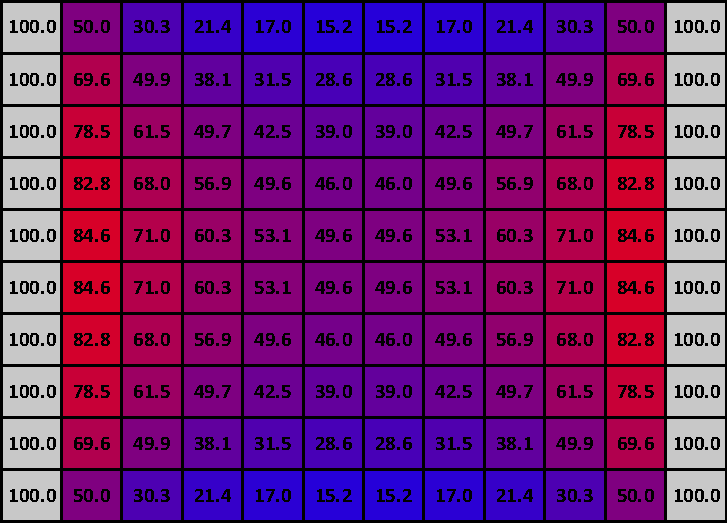
\includegraphics[width=0.6\textwidth]{papers/parallelisierung/images/simulation_10x10_0.135.pdf}
	\caption{Temperaturverteilung für \(10\times 10\)-Gitter, \(\lambda = 0.135\), nach Konvergenz.}
	\label{parallelisierung:fig:simulation_10x10_0.135}
\end{figure}

\paragraph{Fall 2: Instabile Simulation}  
Erhöhen wir die Auflösung auf \(15\times 15\) Messpunkte (\(\Delta l = 0.006\,\mathrm{m}\)), bei gleichem \(\Delta t = 1\,\mathrm{s}\), daraus folgt
\[
\lambda =
10^{-5} \cdot \frac{1}{0.006^2}
\approx 0.376 > \frac14.
\]

Aus diesen Modellparameteren resultierende folgende Temperaturverteilungen.

\begin{figure}[htbp]
	\centering
	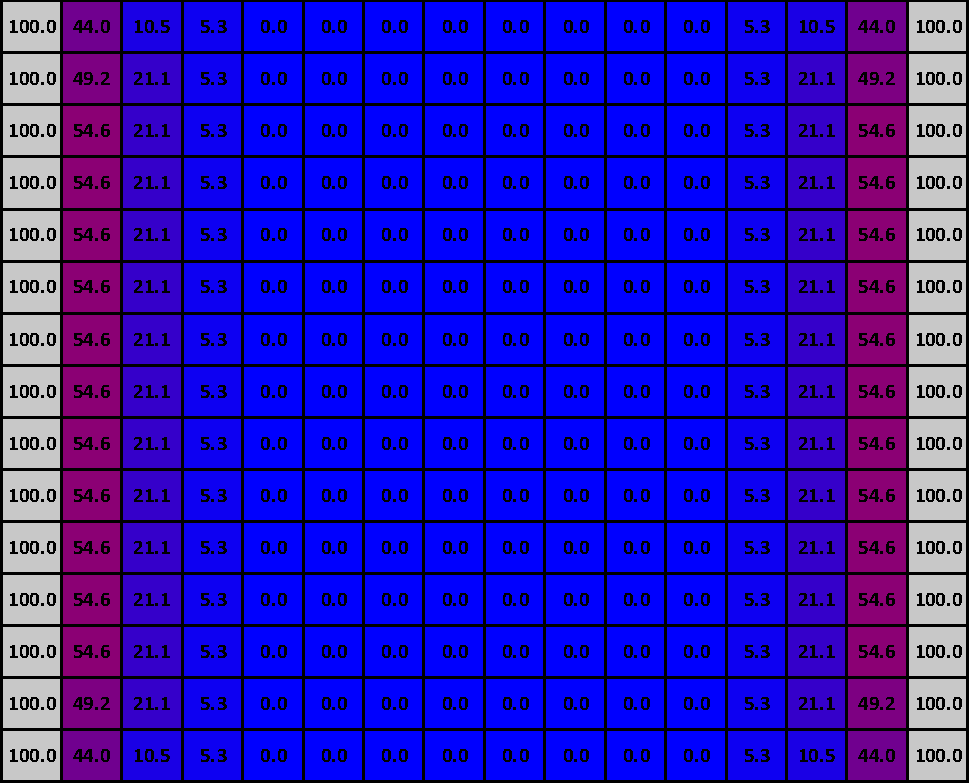
\includegraphics[width=0.6\textwidth]{papers/parallelisierung/images/simulation_15x15_0.376_3it.pdf}
	\caption{\(15\times 15\)-Gitter, \(\lambda = 0.376\), nach 3 Iterationen.}
	\label{parallelisierung:fig:simulation_15x15_0.376_3it}
\end{figure}

\begin{figure}[htbp]
	\centering
	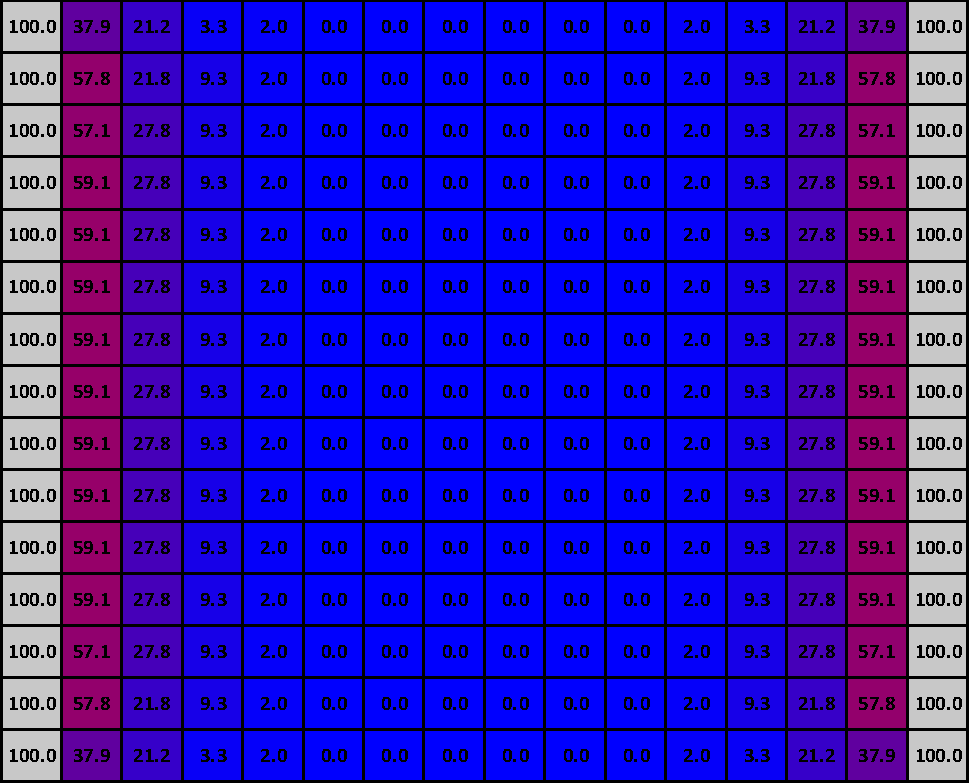
\includegraphics[width=0.6\textwidth]{papers/parallelisierung/images/simulation_15x15_0.376_4it.pdf}
	\caption{\(15\times 15\)-Gitter, \(\lambda = 0.376\), nach 4 Iterationen: erste Instabilitätsartefakte.}
	\label{parallelisierung:fig:simulation_15x15_0.376_4it}
\end{figure}

Zunächst scheint die Simulation noch plausibel (Abbildung~\ref{parallelisierung:fig:simulation_15x15_0.376_3it}), doch bereits nach wenigen Iterationen erscheinen die ersten auffälligen Werte (orange Zahlen in Abbildung~\ref{parallelisierung:fig:simulation_15x15_0.376_4it}). Anhand der physikalischen Intuition sowie den Ergebnissen der stabilen Simulation ist bekannt, dass das Temperaturgefälle von jeder Zelle in der oberen bzw. unteren Hälfte der Metallplatte bei jedem weiteren Schritt nach oben respektive unten (entlang der orangen Pfeile) streng monoton fallend sein muss. Das heißt, es kann nicht plötzlich wieder heißer werden, obwohl wir näher an den Rand gehen. Daraus lässt sich schließen, dass die orange markierten Werte unphysikalisch und somit erste Instabilitäts-Artefakte sind.


Die Ursache lässt sich durch Umformung der Update-Formel verdeutlichen mit
\begin{equation}
	T_{i,j}^{n+1}
	=
	(1-4\lambda)T_{i,j}^n +
	\lambda \left(
	T_{i+1,j}^n + T_{i-1,j}^n + T_{i,j+1}^n + T_{i,j-1}^n
	\right).
\end{equation}
Für \(\lambda > \tfrac14\) wird der Koeffizient \((1-4\lambda)\) negativ was widerum bedeutet das das Zentrum negativ gewichtet wird.  
Dies führt dazu, dass Unterschiede zwischen benachbarten Zellen nicht geglättet, sondern verstärkt werden: es entstehen Über- und Unterschwinger, die sich mit jeder Iteration vergrößern.

\begin{figure}[htbp]
	\centering
	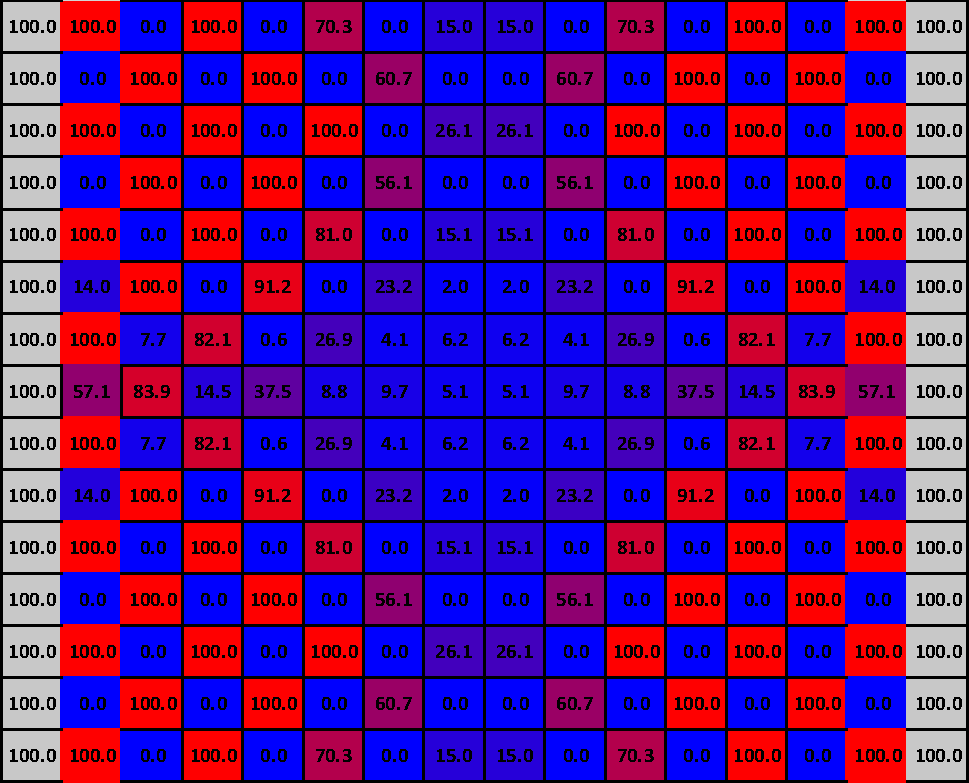
\includegraphics[width=0.6\textwidth]{papers/parallelisierung/images/simulation_15x15_0.376_15it.pdf}
	\caption{\(15\times 15\)-Gitter, \(\lambda = 0.376\), nach 15 Iterationen: klare Instabilitätsartefakte.}
	\label{parallelisierung:fig:simulation_15x15_0.376_15it}
\end{figure}

Lediglich 10 iterationen später zeigt sich das Verhalten gemäss Abbildung~\ref{parallelisierung:fig:simulation_15x15_0.376_15it}, hier ist die Instabilität ser SImulation aufgrund der Verletzung der 2D Stabilitätbedinung mit \(\lambda = 0.376 > \frac{1}{4}\).

\paragraph{Fall 3: Wiederherstellung der Stabilität}  
Durch Verringerung von \(\Delta t\) auf \(0.5\,\mathrm{s}\) ergibt sich
\[
\lambda =
\frac{50}{7850 \cdot 470} \cdot \frac{0.5}{0.006^2}
\approx 0.188 < \frac14,
\]
wodurch die Simulation wieder stabil wird. Die Konvergenz wird nach 315 Iterationen erreicht (Abbildung~\ref{parallelisierung:fig:simulation_15x15_0.188_konv}).

\begin{figure}[htbp]
	\centering
	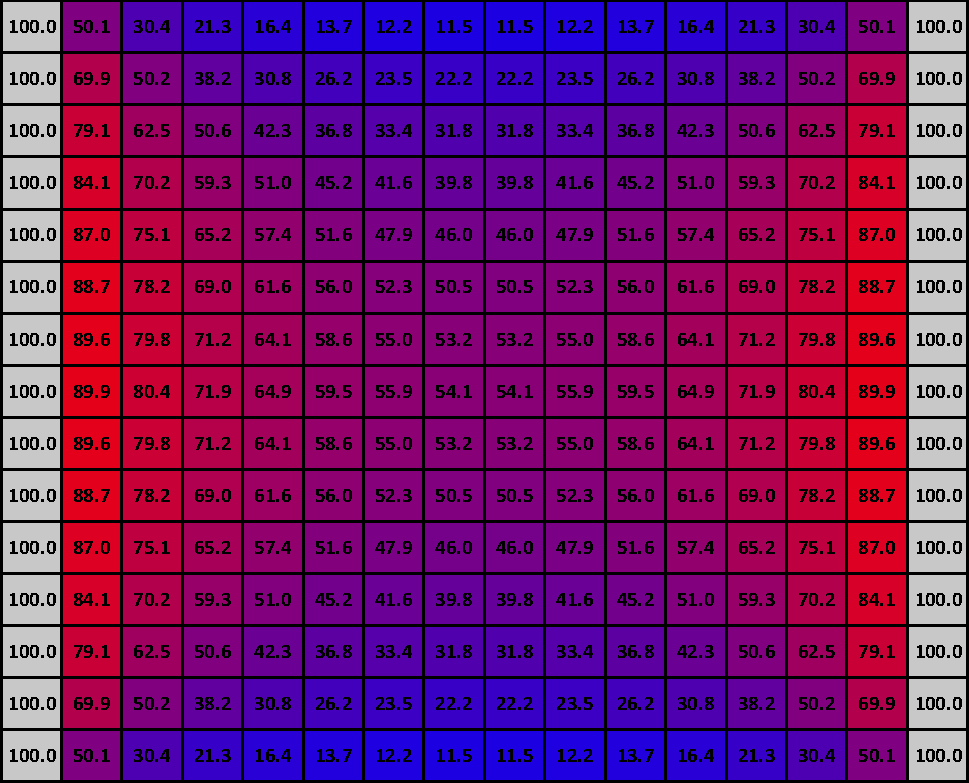
\includegraphics[width=0.6\textwidth]{papers/parallelisierung/images/simulation_15x15_0.188_konv.pdf}
	\caption{\(15\times 15\)-Gitter, \(\lambda = 0.188\), stabil nach Konvergenz.}
	\label{parallelisierung:fig:simulation_15x15_0.188_konv}
\end{figure}
